In this section, we explain how DPC can be applied to this case study. We begin with a description of features $\tX$ and output $\tY$ used for training.

\subsubsection{Training Data} 
\label{SSS:dpc_data}

The fundamental reason why DPC  is suitable for such a problem is that when the complexity rises, there is a huge cost to model all the states given by the dynamical system \eqref{E:bilinear1}. For example, states in the bilinear model also include slab temperatures which require modeling of structural and material properties in detail and often we also need to install new sensors to capture additional states. Thus, DPC is based solely on one state of the model, i.e. the zone temperature that can be easily measured with a thermostat. This serves as the output variable $\tY$ of interest for which we build $N$ trees and $N$ forests as described in Section~\ref{SS:dpcrt} and \ref{SS:dpcrf}, respectively. Therefore, $\tY_{\mathrm{k+j|k}}:=x_{\mathrm{k+j|k}}^1$, where $x^1$ is the first component of $x$.
Next, we define the non-manipulated features $\tX^d_{\mathrm{k|k}}$. At time $k$, for the tree $\mathcal{T}_j$ and the forest $\mathcal{R}_j$, we base these features to include weather disturbances, external disturbances due to occupancy and equipments, and autoregressive terms of the room temperature, i.e.
$\tX^d_{\mathrm{k|k}}:=[ d_{\mathrm{k+j-N|k}} ,\dots,d_{\mathrm{k+j-1|k}}, x_{\mathrm{k|k}}^1,\dots, x_{\mathrm{k-\delta|k}}^1 ]$, where $\delta$ is the order of autoregression.
Finally, the inputs in DPC are exactly same as in MPC. i.e. $\tX^c_{\mathrm{k+j-1|k}}:=u_{\mathrm{k+j-1|k}}$.
The training data in the above format was generated by simulating the bilinear model with rule-based strategies for 10 months in 2007. January and May were deliberately excluded for testing the DPC implementation.
\subsubsection{Optimization} 
\label{SSS:dpc_opt}
For a fair comparison with MPC, we cast DPC optimization problem as follows:

\begin{subequations}
\begin{align}
\text{min } & \sum_{j=1}^{N} ({\tY}_{\mathrm{k+j|k}} - x_{ref}) \mathcal{Q}^{(1,1)} ({\tY}_{\mathrm{k+j|k}} - x_{ref}) + c^T \tX^c_{\mathrm{k+j-1|k}}+  \lambda\epsilon_j\\
\text{s.~t. } & \ \ \ \ \ \tY_{\mathrm{k+j|k}} =  \alpha_j^T \left[1,\tX^c_{\mathrm{k|k}},\dots,\tX^c_{\mathrm{k+j-1|k}} \right]^T \label{SE:dpc}\\
& \ \ \ \ \ \ \ \ \ \ \ \ \ \ \ \underline{\tX}^c \leq \tX^c_{\mathrm{k+j-1|k}} \leq \bar{\tX}^c\\ 
& \ \ \ \ \ \ \ \ \ \ \ \ \underline{\tY}-\epsilon_j \leq \tY_{\mathrm{k+j|k}} \leq \bar{\tY} + \epsilon_j\\\
& \ \ \ \ \ \ \ \ \ \ \ \ \ \ \epsilon_j \geq 0, \ j = 1,\dots,N.
\end{align} \label{E:dpc}
\end{subequations}
\noindent Here $\alpha = \beta$ for DPC-RT and $\alpha = \hat{\Theta}$ for DPC-En.
Note that, \eqref{E:dpc} is DPC analog of \eqref{E:mpc}. The only difference is the state dynamics \eqref{SE:mpc1} and \eqref{SE:mpc2} are now replaced with \eqref{SE:dpc}.

\subsubsection{Validation} 
\label{SSS:dpc_val}

We compare the prediction for the first time step $\tY_{\mathrm{k+1|k}}$ and the 6-hour ahead prediction $\tY_{\mathrm{k+6|k}}$ for a week in the month of May in Figure~\ref{F:validation}. It is visible how trees have a high variance, and the forests are more accurate. Note that data from January and May were not used for training. The quantitative summary of the accuracy is given in Table~\ref{T:validation}. We can see that the random forests are better in all respects.
\begin{table}[h!]
	\centering
	\begin{tabular}{cccc}
		\toprule
		& RMSE & $R^2$ score & EV  \\ 
		\midrule
		tree-$\tY_{\mathrm{k+1|k}}$    &  0.42 &  0.75 & 0.76    \\
		tree-$\tY_{\mathrm{k+6|k}}$  & 0.64 &  0.41  & 0.42 \\
		forest-$\tY_{\mathrm{k+1|k}}$  & 0.29 & 0.87  & 0.88 \\
		forest-$\tY_{\mathrm{k+6|k}}$  & 0.38 & 0.78 & 0.80 \\
		\bottomrule
	\end{tabular}
	\caption{Quantitative comparison of root mean square error (RMSE), $R^2$ score, and explained variance (EV) for trees and forests for different predictions steps.}
	\captionsetup{justification=centering}
	\label{T:validation}
\end{table}

\begin{figure}[h!]
	\centering
	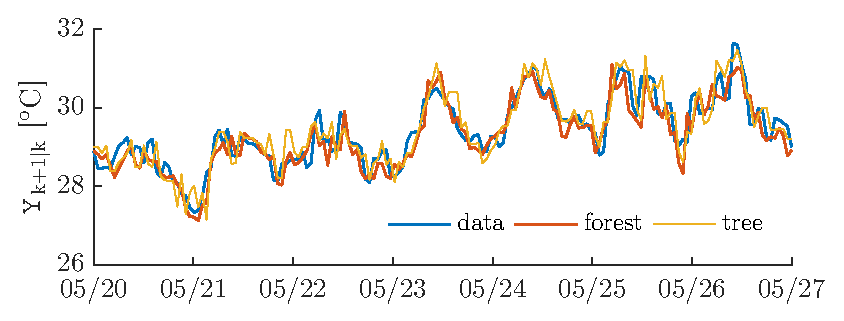
\includegraphics[width=24pc]{figures/validation-s1.eps}
	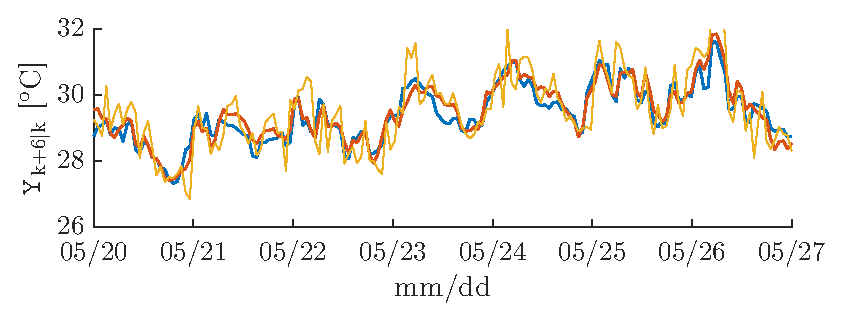
\includegraphics[width=24pc]{figures/validation-s6.eps}
	\caption{Temperature predictions from a tree and a forest for first step prediction (top) and the 6-hour ahead prediction (bottom). Ensemble method shows a relatively higher accuracy.}
	\captionsetup{justification=centering}
	\label{F:validation}
\end{figure}

%\begin{figure}[t!]
%	\centering
%	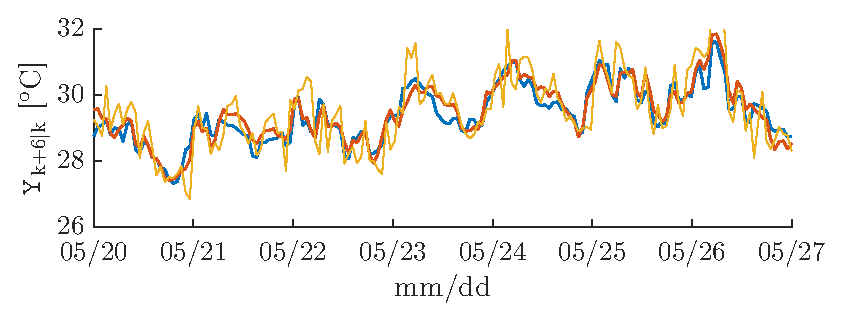
\includegraphics[width=20pc]{figures/validation-s6.eps}
%	\caption{Temperature predictions from a tree and a forest for 6 hour ahead prediction.}
%	\captionsetup{justification=centering}
%	\label{F:validation-s6}
%\end{figure}